\documentclass{amsart} 
\usepackage{amsmath}
\usepackage{verse}
\DeclareMathOperator*{\argmax}{arg\,max}
\DeclareMathOperator*{\argmin}{arg\,min}
\usepackage{graphicx}
\graphicspath{{./}}
\usepackage[fontsize=14pt]{scrextend}
\usepackage{hyperref}
\usepackage{csvsimple}
\usepackage{epigraph}
\title{The Arc of Libery of the World 1220-1800}
\author{Zulfikar Moinuddin Ahmed}
\date{\today}
\begin{document}
\maketitle

\section{Efforts of Bill Gates to Enslave Me}
Bill Gates has revealed in meta his intention to enslave me using various powers that he has acquired, today, April 11 2021.   He claims that my work belongs to him by something called 'White Law'.  Of course he has harmed my Natural Rights and body and health quite a bit, but obviously I am not insane, and I claim Life, Liberty, and Pursuit of Happiness as inviolable and demand that United States either secure them against the transgressions of the criminal Bill Gates or I will demand \$1 trillion in penalty for failure to uphold the promise in every immigration document, which is that United States of America promises to secure my Natural Rights.  

But while this issue is still under consideration, I was quite intrigued by the numerical and geometric patterns of Abolition of Slavery on Earth in history.  Bill Gates, being quite undereducated and illiterate, does not appreciate the greatness of the advance of end of slavery across the globe.  

My own education was quite a bit better than Bill Gates' since I attended Princeton after having completed High School in New York and graduated valedictorian of my class in 1991, with a few thousand multi-ethnic student body.  My grades in American history honours courses were satisfactory and my intuition that "slavery ended mostly in nineteenth century" was correct.  Since I was born in 1973 and graduated high school in 1991, I did not ever think that Slavery was even an interesting concept any more.  But since Bill Gates is trying so hard to go against all of history by enslaving me, which is quite amusing to me because my intellectual stature in history is so much greater than his. But my dear readers will not be as interested in this and be much more interested in the {\em Ark of Liberty}.

I named a geographic region in Eurasia the {\em Ark of Liberty}.  This spans some parts of Western and Northern Europe to Russia and then a stretch of East Asia.  Laws banning Slavery in this ark are the earliest, from 1220 to 1800, before the nineteenth century.  This made me rather curious, that Man developed Liberty as a {\em principle} before the nineteenth century.  The example of various 'convictions' of Bill Gates for his 'white right' to enslave me I personally dismiss with a wave of my hands, because my convictions of Natural Right of Liberty for all human beings is far more advanced and superior.  But the question is what is the history of my own conviction?  Yes, yes, I cannot even bear the thought of all sorts of my beloved people, the Human Race being enslaved.  Obviously Human Beings are not born on Earth to be enslaved.  If people were born to be enslaved then no one would have any deep desire to be free, but everyone -- even those who want to enslave -- long for freedom and liberty {\em for themselves} and cook up various fairy tales about others do not have a right to be free because of some fiction or other.  It's wrong.  If you believe any of this, you are simply dull and wrong and ought to correct your viewpoint.

Now let's actuall take a look at this beautiful Ark of Liberty.

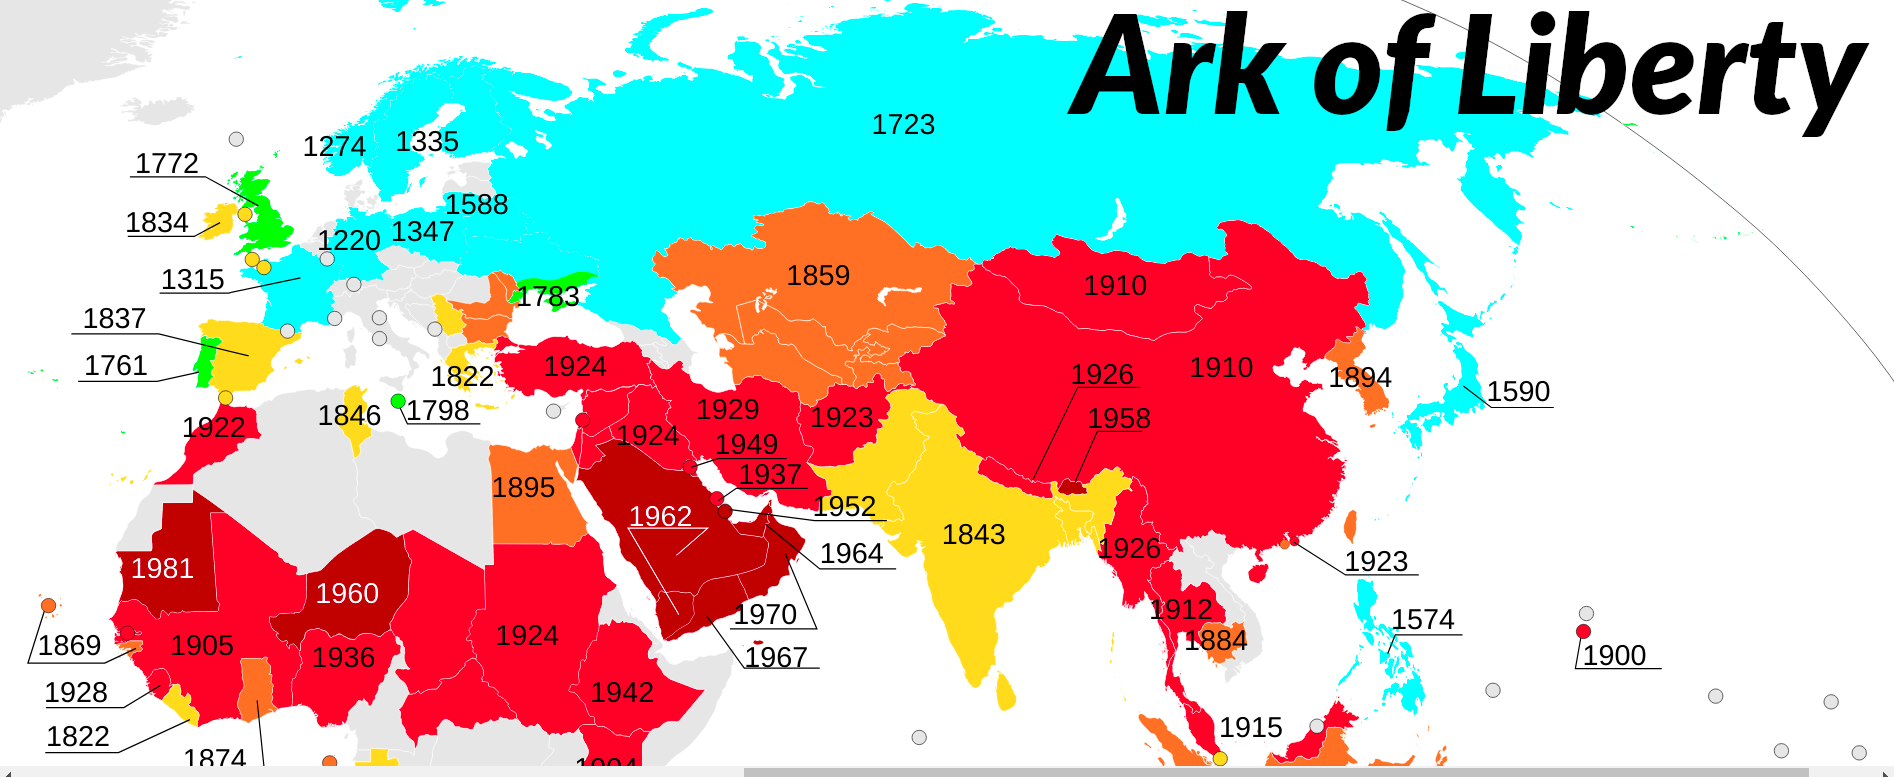
\includegraphics[scale=
0.2]{libertyark.png}

\section{Japan 1590 Abolition}

Japanese Toyotomi Hideyoshi bans slavery except as punishment for criminals in 1590.  Now John Locke comes into the scene 29 August 1632 – 28 October 1704.  This is quite intriguing, for here was a man abolishing slavery withou influence of John Locke.

For me, there is a deep mystery regarding Liberty and Human Nature.  

\section{To What Extent is Liberty Human Nature?}

We know today that Autonomy is more necessary than Money for Human Well-Being.  You can see my note on place of money in your life.  We can deduce that Autonomy Needs are part of Human Nature from work of Tay-Diener.  What is interesting in history is to understand to what extent this was implicitly known in history.  Japan's abolition of slavery in 1590 does come later than 873 when Pope John VIII considers enslavements of Christians a sin.  In Islam one had, "According to Patrick Manning, the Islamic legislations against the abuse of the slaves limited the extent of enslavement in Arabian peninsula and to a lesser degree for the whole area of the whole Umayyad Caliphate where slavery existed since the most ancient times."  Umayyad was 661–750 CE.

The history of abolition of slavery goes earlier to events in Greece, Rome, China.  

\section{Autonomy as Psychological Need is New}

We can see that both in Christianity and Islam there was a drive against slavery. Here I can contribute by adding that Autonomy Needs are part of Universal Human Nature and therefore laws securing Natural Right of Liberty are actually deeper than artificial laws but tap into Universal Human Nature.  Previous to my examination, there was not a clear understanding of Universal Psychological Need that has no exceptions in the Human Race for well-being.  What we see in history is a confusion that leads to heroic abolition from political considerations rather than simpler deductions from Human Nature.

\section{Epilogue}

It is rare for anyone at all to gain the privilege of being at the center of action of the entire world.  And I am quite able to perform in this nexus.  I learn from Emerson that great men, such as myself, accept childlike the spirit of the age.  The foolish Bill Gates, despite repeated warnings, despite repeated figures that 78% of Earth today accept the importance of protecting human rights, dares to attempt to use his paltry powers to enslave me. I, who am far greater than Bill Gates in my Ancient Aristocracy; I, who am far more immortal in my Genius than him.  I want to quickly create a dataset of when slavery was abolished in the various countries around the world, to tell you just how pathetically retrogressive he is.  The dilettante without education enough to understand the flow of history, the petulant man-child who dares to disturb the Life, Liberty and Pursuit of Happiness of one of the greatest geniuses that the Human Race has produced, one who had sat beneath the walls of Union Square Theater and walked among the lowest of the dead.  I take position now with the Angel of History behind me, and the vast future.  Foolish is the man who is unable to see the winds of history and allows his Hubris to consider going against them.  His ship is headed for the rocks.  


\begin{verse}
Bill Gates the sailor, a fortnight dead,\\
Forgot the cry of gulls, and the deep sea swell\\
And the profit and loss.\\
                           A current under sea\\
Picked his bones in whispers. \\
As he rose and fell\\
He passed the stages of his age and youth\\
Entering the whirlpool.\\
                                 Gentile or Jew\\
O you who turn the wheel and look to windward,\\
Consider Bill Gates, who was once handsome and tall as you.

\end{verse}

\end{document}

